\chapter{Implementazioni in LiSA}\label{chapter:lisa}



LiSA (\textbf{Li}brary for \textbf{S}tatic \textbf{A}nalysis) è un framework generico sviluppato come libreria open-source in Java che permette in modo facile, diretto e completo l'analisi statica tramite interpretazione astratta di semplici programmi multi linguaggio. Una basilare rappresentazione del flow dell'analisi in LiSA può essere vista in figura \ref{fig:lisaAnalysisFlow} e lo possiamo riassumere così: (1) un programma scritto in un linguaggio L viene passato al front-end appropriato che lo trascrive nel linguaggio intermedio compreso da LiSA basato su Control Flow Graph (generalmente un LiSA CFG per funzione), (2) LiSA poi analizza i CFGs creati con un algoritmo di ricerca del fix-point seguendo le linee guida passate da utente tramite la configurazione (ad esempio: domini da usare, parametri per l'algorito del fix-point, tipo di analisi interprocedurale), (3) infine LiSA esegue i semantics checks, anch'essi passati da utente, ed eventualmente genera warnings ed errori se l'analisi non ne rispetta i vincoli. 

LiSA mette a disposizione: (i) un linguaggio interno basato su control-flow graph estensibile e abbastanza generico da supportare i costrutti semantici di molti linguaggi di programmazione, (ii) una vasta gamma di front-end per la traduzione di programmi in LiSA CFGs, (iii) una base comune per lo sviluppo di nuovi domini astratti da usare nelle analisi (sia relazionali che non, più alcuni domini built-in) ed infine (iv) un algoritmo per il calcolo del fix-point dei LiSA CFGs con metodo di risoluzione basato su working-set list.

Durante la mia tesi ho lavorato soprattutto sulle componenti (iii) e (iv). Per prima cosa ho esteso l'algoritmo per il calcolo del fix-point affinchè fosse in grado di eseguire anche la fase discendente partendo da un post-fix-point precedentemente calcolato, ho aggiunto classi generiche come base per l'implementazione del dominio astratto degli insiemi non ridondanti di un altro dominio astratto (nonchè una implementazione concreta di ciò per gli intervalli) ed infine, per scopo sperimentale, una rudimentale versione del decoupling capace di usare domini diversi per salire e scendere nell'analisi.

\begin{figure}
    \centering
\usetikzlibrary{shadows}
\tikzset{every picture/.style={line width=0.75pt}} %set default line width to 0.75pt   
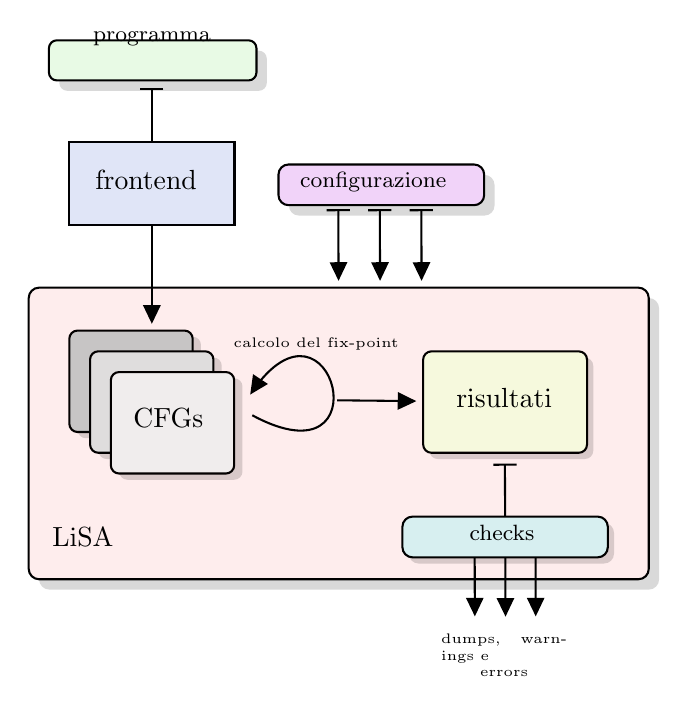
\begin{tikzpicture}[x=0.75pt,y=0.75pt,yscale=-1,xscale=1]
%uncomment if require: \path (0,336); %set diagram left start at 0, and has height of 336

%Shape: Rectangle [id:dp735576293814507] 
\draw  [color={rgb, 255:red, 0; green, 0; blue, 0 }  ,draw opacity=1 ][fill={rgb, 255:red, 254; green, 237; blue, 237 }  ,fill opacity=1 ][general shadow={fill={rgb, 255:red, 0; green, 0; blue, 0 }  ,shadow xshift=3.75pt,shadow yshift=-3.75pt, opacity=0.15 }] (10.44,145) .. controls (10.44,142.24) and (12.68,140) .. (15.44,140) -- (304.17,140) .. controls (306.93,140) and (309.17,142.24) .. (309.17,145) -- (309.17,275.5) .. controls (309.17,278.26) and (306.93,280.5) .. (304.17,280.5) -- (15.44,280.5) .. controls (12.68,280.5) and (10.44,278.26) .. (10.44,275.5) -- cycle ;
%Straight Lines [id:da23563586478588427] 
\draw    (69.77,44.13) -- (69.77,154.4) ;
\draw [shift={(69.77,157.4)}, rotate = 270] [fill={rgb, 255:red, 0; green, 0; blue, 0 }  ][line width=0.08]  [draw opacity=0] (8.93,-4.29) -- (0,0) -- (8.93,4.29) -- cycle    ;
\draw [shift={(69.77,44.13)}, rotate = 270] [color={rgb, 255:red, 0; green, 0; blue, 0 }  ][line width=0.75]    (0,5.59) -- (0,-5.59)   ;
%Shape: Rectangle [id:dp6301022803478207] 
\draw  [color={rgb, 255:red, 0; green, 0; blue, 3 }  ,draw opacity=1 ][fill={rgb, 255:red, 224; green, 229; blue, 247 }  ,fill opacity=1 ] (30,70) -- (109.57,70) -- (109.57,110) -- (30,110) -- cycle ;
%Rounded Rect [id:dp2844998293479686] 
\draw  [fill={rgb, 255:red, 232; green, 250; blue, 229 }  ,fill opacity=1 ][general shadow={fill={rgb, 255:red, 0; green, 0; blue, 0 }  ,shadow xshift=3.75pt,shadow yshift=-3.75pt, opacity=0.15 }] (20.17,24.7) .. controls (20.17,22.56) and (21.9,20.83) .. (24.03,20.83) -- (116.3,20.83) .. controls (118.44,20.83) and (120.17,22.56) .. (120.17,24.7) -- (120.17,36.3) .. controls (120.17,38.44) and (118.44,40.17) .. (116.3,40.17) -- (24.03,40.17) .. controls (21.9,40.17) and (20.17,38.44) .. (20.17,36.3) -- cycle ;
%Rounded Rect [id:dp015147798185889627] 
\draw  [fill={rgb, 255:red, 241; green, 211; blue, 249 }  ,fill opacity=1 ][general shadow={fill={rgb, 255:red, 0; green, 0; blue, 0 }  ,shadow xshift=3.75pt,shadow yshift=-3.75pt, opacity=0.15 }] (130.78,85.5) .. controls (130.78,82.83) and (132.94,80.67) .. (135.61,80.67) -- (225.03,80.67) .. controls (227.7,80.67) and (229.87,82.83) .. (229.87,85.5) -- (229.87,95.43) .. controls (229.87,98.1) and (227.7,100.27) .. (225.03,100.27) -- (135.61,100.27) .. controls (132.94,100.27) and (130.78,98.1) .. (130.78,95.43) -- cycle ;
%Shape: Rectangle [id:dp3167426310658905] 
\draw  [color={rgb, 255:red, 3; green, 0; blue, 0 }  ,draw opacity=1 ][fill={rgb, 255:red, 199; green, 197; blue, 197 }  ,fill opacity=1 ][general shadow={fill={rgb, 255:red, 0; green, 0; blue, 0 }  ,shadow xshift=3pt,shadow yshift=-2.25pt, opacity=0.15 }] (30,164.67) .. controls (30,162.46) and (31.79,160.67) .. (34,160.67) -- (85.44,160.67) .. controls (87.65,160.67) and (89.44,162.46) .. (89.44,164.67) -- (89.44,205.56) .. controls (89.44,207.76) and (87.65,209.56) .. (85.44,209.56) -- (34,209.56) .. controls (31.79,209.56) and (30,207.76) .. (30,205.56) -- cycle ;
%Shape: Rectangle [id:dp5390943849837029] 
\draw  [color={rgb, 255:red, 3; green, 0; blue, 0 }  ,draw opacity=1 ][fill={rgb, 255:red, 246; green, 249; blue, 221 }  ,fill opacity=1 ][general shadow={fill={rgb, 255:red, 0; green, 0; blue, 0 }  ,shadow xshift=2.25pt,shadow yshift=-2.25pt, opacity=0.15 }] (200.48,174.7) .. controls (200.48,172.49) and (202.27,170.7) .. (204.48,170.7) -- (275.44,170.7) .. controls (277.65,170.7) and (279.44,172.49) .. (279.44,174.7) -- (279.44,215.56) .. controls (279.44,217.76) and (277.65,219.56) .. (275.44,219.56) -- (204.48,219.56) .. controls (202.27,219.56) and (200.48,217.76) .. (200.48,215.56) -- cycle ;
%Shape: Rectangle [id:dp6482074079685427] 
\draw  [color={rgb, 255:red, 3; green, 0; blue, 0 }  ,draw opacity=1 ][fill={rgb, 255:red, 223; green, 221; blue, 221 }  ,fill opacity=1 ][general shadow={fill={rgb, 255:red, 0; green, 0; blue, 0 }  ,shadow xshift=3pt,shadow yshift=-2.25pt, opacity=0.15 }] (40,174.67) .. controls (40,172.46) and (41.79,170.67) .. (44,170.67) -- (95.44,170.67) .. controls (97.65,170.67) and (99.44,172.46) .. (99.44,174.67) -- (99.44,215.56) .. controls (99.44,217.76) and (97.65,219.56) .. (95.44,219.56) -- (44,219.56) .. controls (41.79,219.56) and (40,217.76) .. (40,215.56) -- cycle ;
%Shape: Rectangle [id:dp5665391899993595] 
\draw  [color={rgb, 255:red, 3; green, 0; blue, 0 }  ,draw opacity=1 ][fill={rgb, 255:red, 240; green, 237; blue, 237 }  ,fill opacity=1 ][general shadow={fill={rgb, 255:red, 0; green, 0; blue, 0 }  ,shadow xshift=3pt,shadow yshift=-2.25pt, opacity=0.15 }] (50,184.67) .. controls (50,182.46) and (51.79,180.67) .. (54,180.67) -- (105.44,180.67) .. controls (107.65,180.67) and (109.44,182.46) .. (109.44,184.67) -- (109.44,225.56) .. controls (109.44,227.76) and (107.65,229.56) .. (105.44,229.56) -- (54,229.56) .. controls (51.79,229.56) and (50,227.76) .. (50,225.56) -- cycle ;
%Straight Lines [id:da034591409315066324] 
\draw [line width=0.75]    (159.61,102.69) -- (159.71,133.69) ;
\draw [shift={(159.72,136.69)}, rotate = 269.81] [fill={rgb, 255:red, 0; green, 0; blue, 0 }  ][line width=0.08]  [draw opacity=0] (8.93,-4.29) -- (0,0) -- (8.93,4.29) -- cycle    ;
\draw [shift={(159.61,102.69)}, rotate = 269.81] [color={rgb, 255:red, 0; green, 0; blue, 0 }  ][line width=0.75]    (0,5.59) -- (0,-5.59)   ;
%Straight Lines [id:da8442899163237636] 
\draw [line width=0.75]    (179.61,102.69) -- (179.71,133.69) ;
\draw [shift={(179.72,136.69)}, rotate = 269.81] [fill={rgb, 255:red, 0; green, 0; blue, 0 }  ][line width=0.08]  [draw opacity=0] (8.93,-4.29) -- (0,0) -- (8.93,4.29) -- cycle    ;
\draw [shift={(179.61,102.69)}, rotate = 269.81] [color={rgb, 255:red, 0; green, 0; blue, 0 }  ][line width=0.75]    (0,5.59) -- (0,-5.59)   ;
%Straight Lines [id:da1808180600514191] 
\draw [line width=0.75]    (199.61,102.69) -- (199.71,133.69) ;
\draw [shift={(199.72,136.69)}, rotate = 269.81] [fill={rgb, 255:red, 0; green, 0; blue, 0 }  ][line width=0.08]  [draw opacity=0] (8.93,-4.29) -- (0,0) -- (8.93,4.29) -- cycle    ;
\draw [shift={(199.61,102.69)}, rotate = 269.81] [color={rgb, 255:red, 0; green, 0; blue, 0 }  ][line width=0.75]    (0,5.59) -- (0,-5.59)   ;
%Curve Lines [id:da7168976803847669] 
\draw    (118.17,201.5) .. controls (182.52,236.15) and (156.7,134.57) .. (118.33,189.78) ;
\draw [shift={(117.17,191.5)}, rotate = 303.47] [fill={rgb, 255:red, 0; green, 0; blue, 0 }  ][line width=0.08]  [draw opacity=0] (8.93,-4.29) -- (0,0) -- (8.93,4.29) -- cycle    ;
%Straight Lines [id:da3343995640969275] 
\draw [line width=0.75]    (159,194.28) -- (194.17,194.64) ;
\draw [shift={(197.17,194.67)}, rotate = 180.58] [fill={rgb, 255:red, 0; green, 0; blue, 0 }  ][line width=0.08]  [draw opacity=0] (8.93,-4.29) -- (0,0) -- (8.93,4.29) -- cycle    ;
%Straight Lines [id:da6598443106986112] 
\draw [line width=0.75]    (239.87,225.3) -- (240.16,295.5) ;
\draw [shift={(240.17,298.5)}, rotate = 269.76] [fill={rgb, 255:red, 0; green, 0; blue, 0 }  ][line width=0.08]  [draw opacity=0] (8.93,-4.29) -- (0,0) -- (8.93,4.29) -- cycle    ;
\draw [shift={(239.87,225.3)}, rotate = 269.76] [color={rgb, 255:red, 0; green, 0; blue, 0 }  ][line width=0.75]    (0,5.59) -- (0,-5.59)   ;
%Rounded Rect [id:dp7910872057944298] 
\draw  [fill={rgb, 255:red, 215; green, 239; blue, 240 }  ,fill opacity=1 ][general shadow={fill={rgb, 255:red, 0; green, 0; blue, 0 }  ,shadow xshift=2.25pt,shadow yshift=-2.25pt, opacity=0.15 }] (190.5,255.17) .. controls (190.5,252.5) and (192.66,250.33) .. (195.33,250.33) -- (284.61,250.33) .. controls (287.28,250.33) and (289.44,252.5) .. (289.44,255.17) -- (289.44,265.1) .. controls (289.44,267.77) and (287.28,269.93) .. (284.61,269.93) -- (195.33,269.93) .. controls (192.66,269.93) and (190.5,267.77) .. (190.5,265.1) -- cycle ;
%Straight Lines [id:da7891879484603097] 
\draw [line width=0.75]    (254.64,270.28) -- (254.71,295.36) ;
\draw [shift={(254.72,298.36)}, rotate = 269.83] [fill={rgb, 255:red, 0; green, 0; blue, 0 }  ][line width=0.08]  [draw opacity=0] (8.93,-4.29) -- (0,0) -- (8.93,4.29) -- cycle    ;
%Straight Lines [id:da9550393969063078] 
\draw [line width=0.75]    (225.31,270.28) -- (225.38,295.36) ;
\draw [shift={(225.39,298.36)}, rotate = 269.83] [fill={rgb, 255:red, 0; green, 0; blue, 0 }  ][line width=0.08]  [draw opacity=0] (8.93,-4.29) -- (0,0) -- (8.93,4.29) -- cycle    ;

% Text Node
\draw (59.33,197) node [anchor=north west][inner sep=0.75pt]   [align=left] {CFGs};
% Text Node
\draw (139.67,83) node [anchor=north west][inner sep=0.75pt]   [align=left] {{\footnotesize configurazione}};
% Text Node
\draw (38.67,15.25) node [anchor=north west][inner sep=0.75pt]  [font=\footnotesize] [align=left] {\begin{minipage}[lt]{44.44pt}\setlength\topsep{0pt}
\begin{center}
programma
\end{center}

\end{minipage}};
% Text Node
\draw (41,82) node [anchor=north west][inner sep=0.75pt]   [align=left] {frontend};
% Text Node
\draw (20.33,254) node [anchor=north west][inner sep=0.75pt]   [align=left] {LiSA};
% Text Node
\draw (107.67,162.75) node [anchor=north west][inner sep=0.75pt]  [font=\tiny] [align=left] {calcolo del fix-point};
% Text Node
\draw (215,187) node [anchor=north west][inner sep=0.75pt]   [align=left] {risultati};
% Text Node
\draw (221.33,253.08) node [anchor=north west][inner sep=0.75pt]   [align=left] {{\footnotesize checks}};
% Text Node
\draw (207.67,305.42) node [anchor=north west][inner sep=0.75pt]  [font=\tiny] [align=left] {\begin{minipage}[lt]{45.52pt}\setlength\topsep{0pt}
dumps, warnings e
\begin{center}
errors
\end{center}

\end{minipage}};


\end{tikzpicture}
    \caption{Schema del flow dell'analisi in LiSA}
    \label{fig:lisaAnalysisFlow}
\end{figure}

\section{LiSA}
In questa sezione faremo una overview della archutettura di LiSA focalizzandoci sulla struttura della rappresentazione interna dei programmi, sulle interfacce attraverso cui è possibile definire nuovi domini astratti e sull'organizzazione della vera e propria analisi statica (andando a guardarne le componenti e gli algoritmi).

\subsection{I CFG di LiSA}
La struttura dei CFG in LiSA è progettata per essere il più flessibile possibile così da essere in grado di rappresentare il maggior numero di costrutti semantici provenienti da più linguaggi di programmazione. Un LiSA CFG ha gli \texttt{Statement} come nodi (ognuno con il proprio significato semantico) e gli \texttt{Edge} come archi (i quali modellano il flusso di dati durante l'esecuzione del programma). 

\subsubsection{\texttt{Statement}}
Uno \texttt{Statement} rappresenta un costrutto semantico base di un linguaggio di programmazione che non modifica il flusso di esecuzione. Uno \texttt{Statement} che lascia un valore sullo stack è detto \texttt{Expression}, che è una sotto classe di \texttt{Statement}. La maggior parte delle \texttt{Expression} rappresentano operazioni base comuni a molti linguaggio (come addizione, sottrazione, e tutte le altre operazioni aritmetiche, operazioni sulle stringhe come concatenazione o lunghezza, operazioni logiche su booleani come and e or e così via). Una sotto-classe particolare di \texttt{Expression} è \texttt{Call}. Esistono molti tipi di \texttt{Call} in LiSA, ma riassuntivamente queste rappresentano chiamate ad altre funzioni, quindi altri CFG. Le \texttt{Call} vengono gestite tramite una classe che implementa l'interfaccia \texttt{InterproceduralAnalysis}, il compito di una di queste classi è proprio di gestire l'interproceduralità di un programma, ovvero la possibilità di avere, in una funzione, chiamate ad altre funzioni (o a se stesse, quindi chiamate ricorsive). In figura \ref{fig:gerarchiaStatement} si può vedere una sommaria e non completa gerarchia della classe \texttt{Statement}.

\begin{figure}[ht]
	\centering
	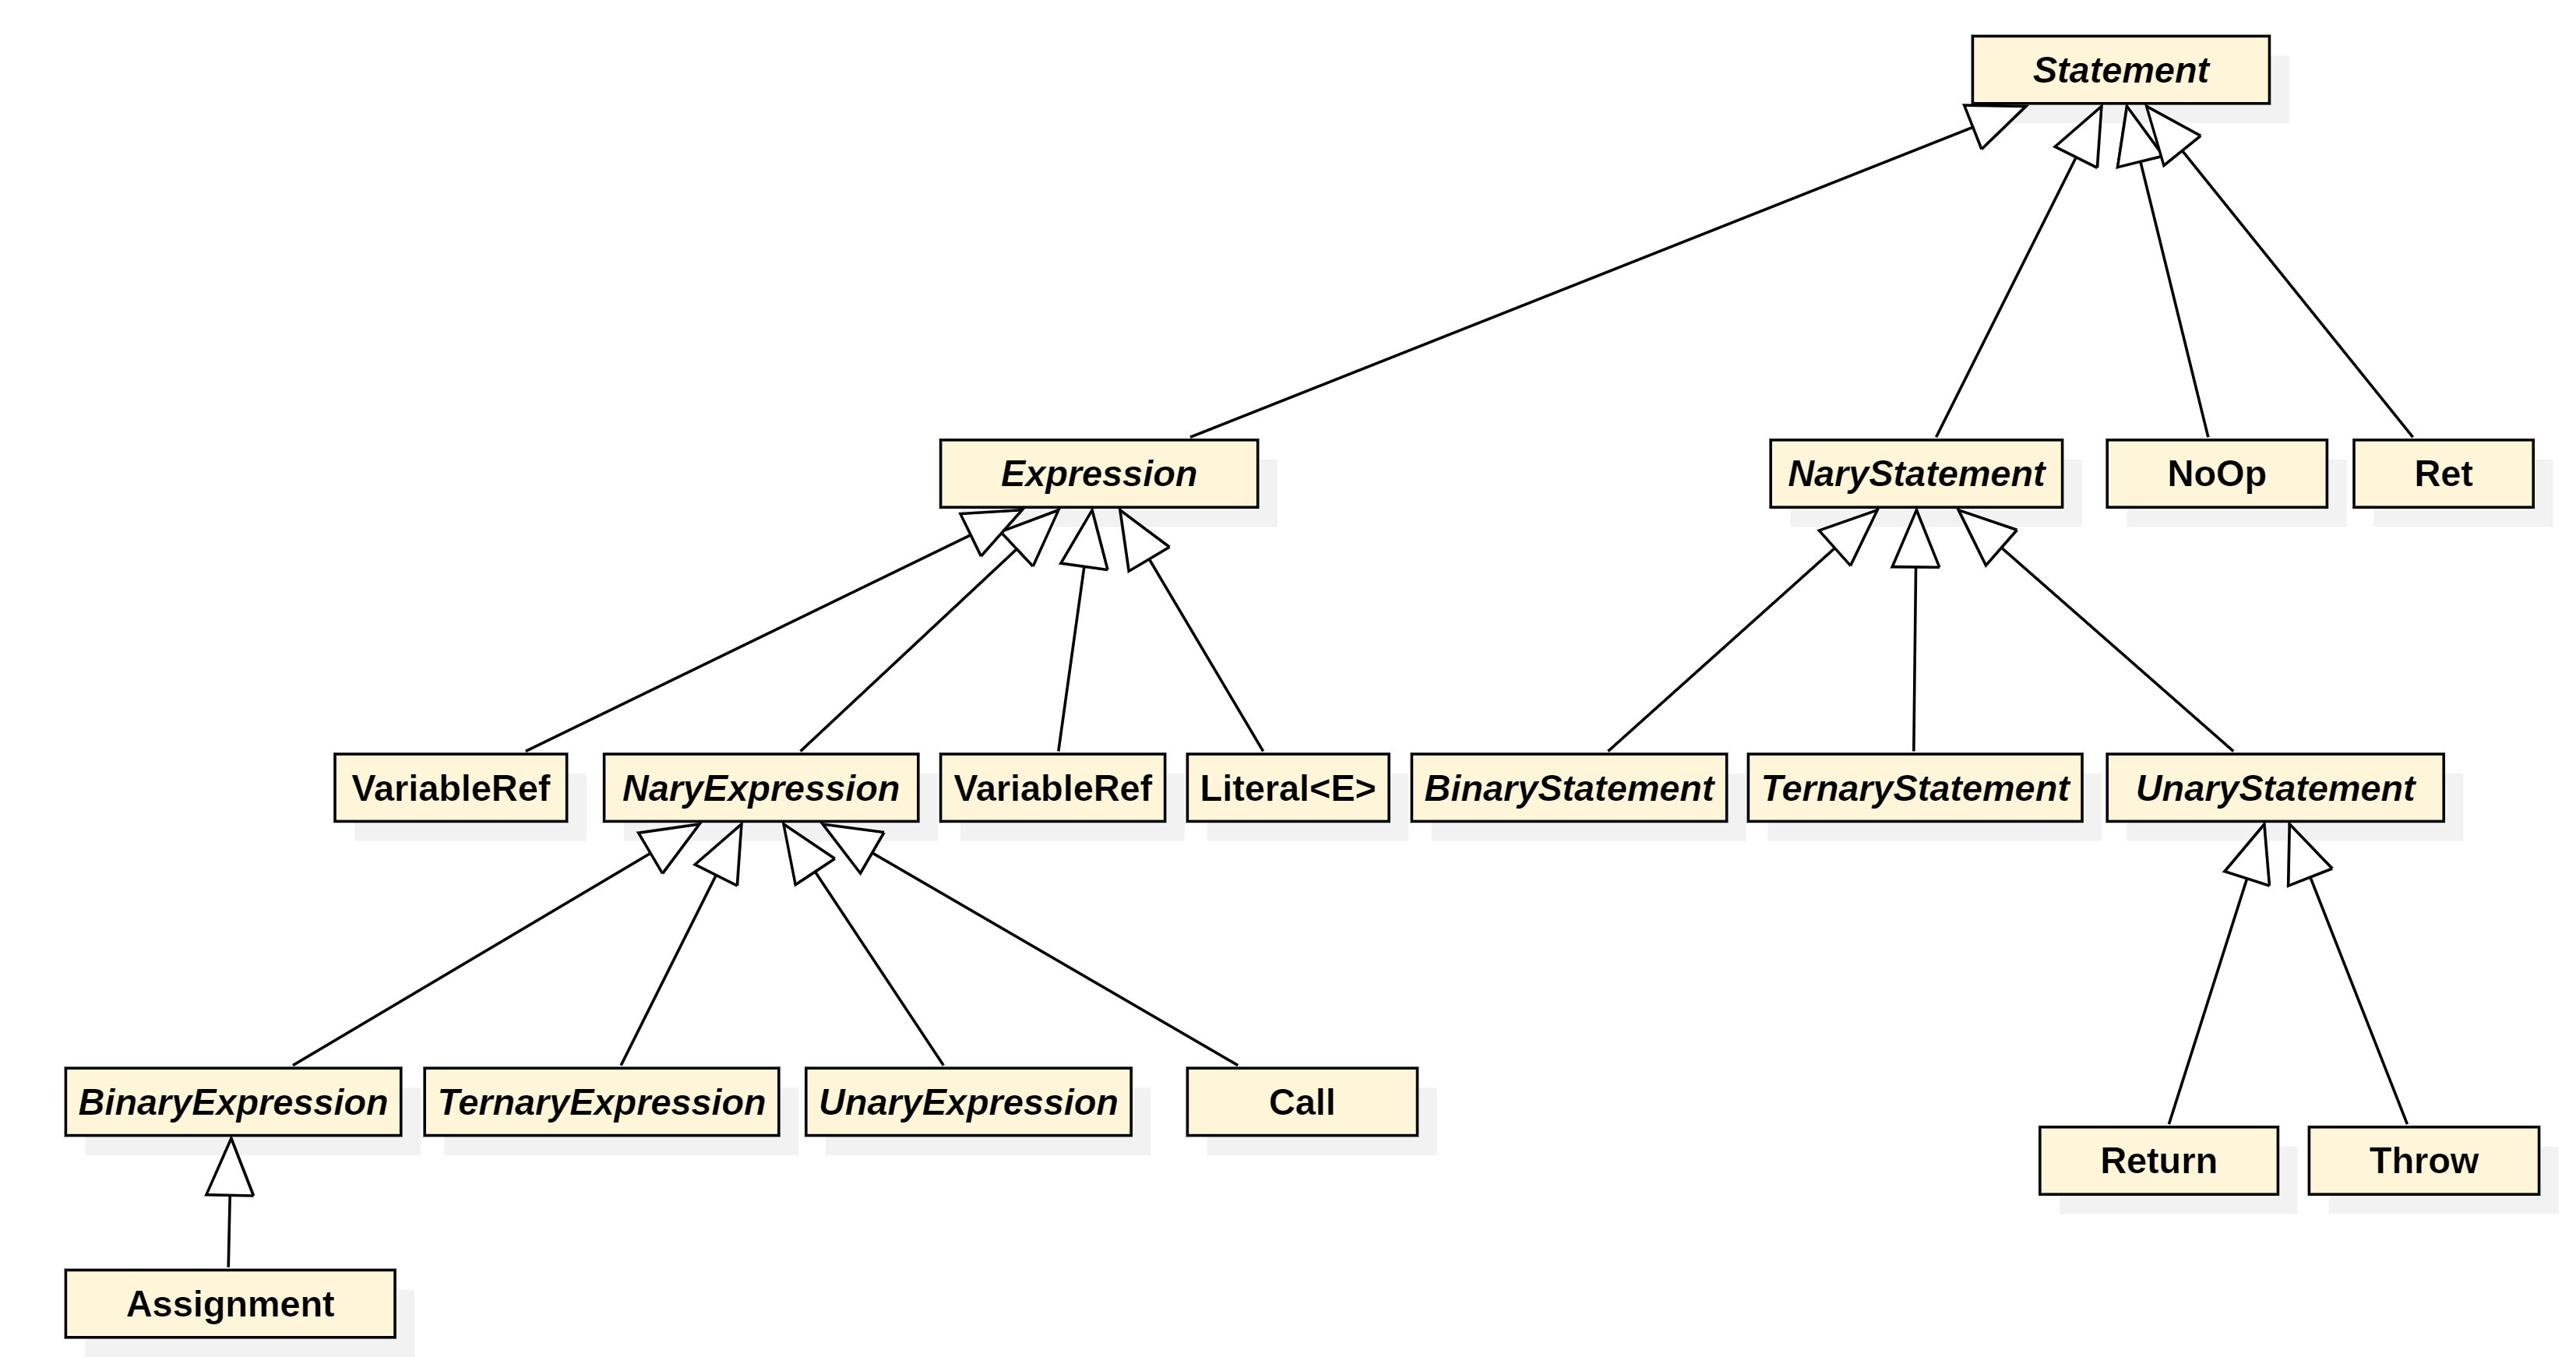
\includegraphics[width=0.9\textwidth]{Immagini/gerarchiaStatement.png}
	\caption{Gerarchia della classe \texttt{statement}}
	\label{fig:gerarchiaStatement}
\end{figure}

\subsubsection{\texttt{Edge}}
La classe \texttt{Edge} collega tra di loro due nodi. Esistono tre tipi di \texttt{Edge}: \texttt{SequentialEdge}, modella un flusso senza condizione e sequenziale dal nodo di origine al nodo target, \texttt{TrueEdge}, modella un flusso condizionale se la condizione nel nodo di origine è vera, \texttt{FalseEdge}, modella un flusso condizionale se la condizione nel nodo di origine è falsa.
\\

\texttt{Edge} e \texttt{Statement} modificano le istanze del dominio astratto attraverso, rispettivamente, i metodi \texttt{traverse}, che agisce sul post-state del nodo di origine e consegna il valore trasformato al pre-state del nodo target, e \texttt{semantics}, che trasforma il pre-state di un nodo nel suo post-state. Più precisamente però non è la classe \texttt{Statement} che modifica il dominio astratto, infatti ogni \texttt{Statement} viene trascritto in una composizione di \texttt{SymbolicExpression} a run-time durante l'analisi. Ogni \texttt{SymbolicExpression} ha un significato semantico ben preciso e le istanze del dominio astratto definiscono gli effetti semantici su quest'ultime e non sugli \texttt{Statement}. Possiamo vedere gli \texttt{Statement} come la sintassi e le \texttt{SymbolicExpression} come la semantica dei CFG in LiSA. Le \texttt{SymbolicExpression} si dividono in due principali tipi di espressione, abbiamo le \texttt{HeapExpression}, ovvero le espressioni che modellano le operazioni sul'heap (come \texttt{HeapAllocation}, \texttt{AccessChild}), e le \texttt{ValueExpression}, che modellano modifiche e operazione sul valore di variabili e costanti (qui per esempio abbiamo \texttt{Addition}, \texttt{LessOrEqual}, \texttt{And}, \texttt{Modulo}, etc..). In figura \ref{fig:gerarchiaSymbolic} qua sotto si vede la non completa gerarchia delle \texttt{SymbolicExpression}.

\begin{figure}[ht]
	\centering
	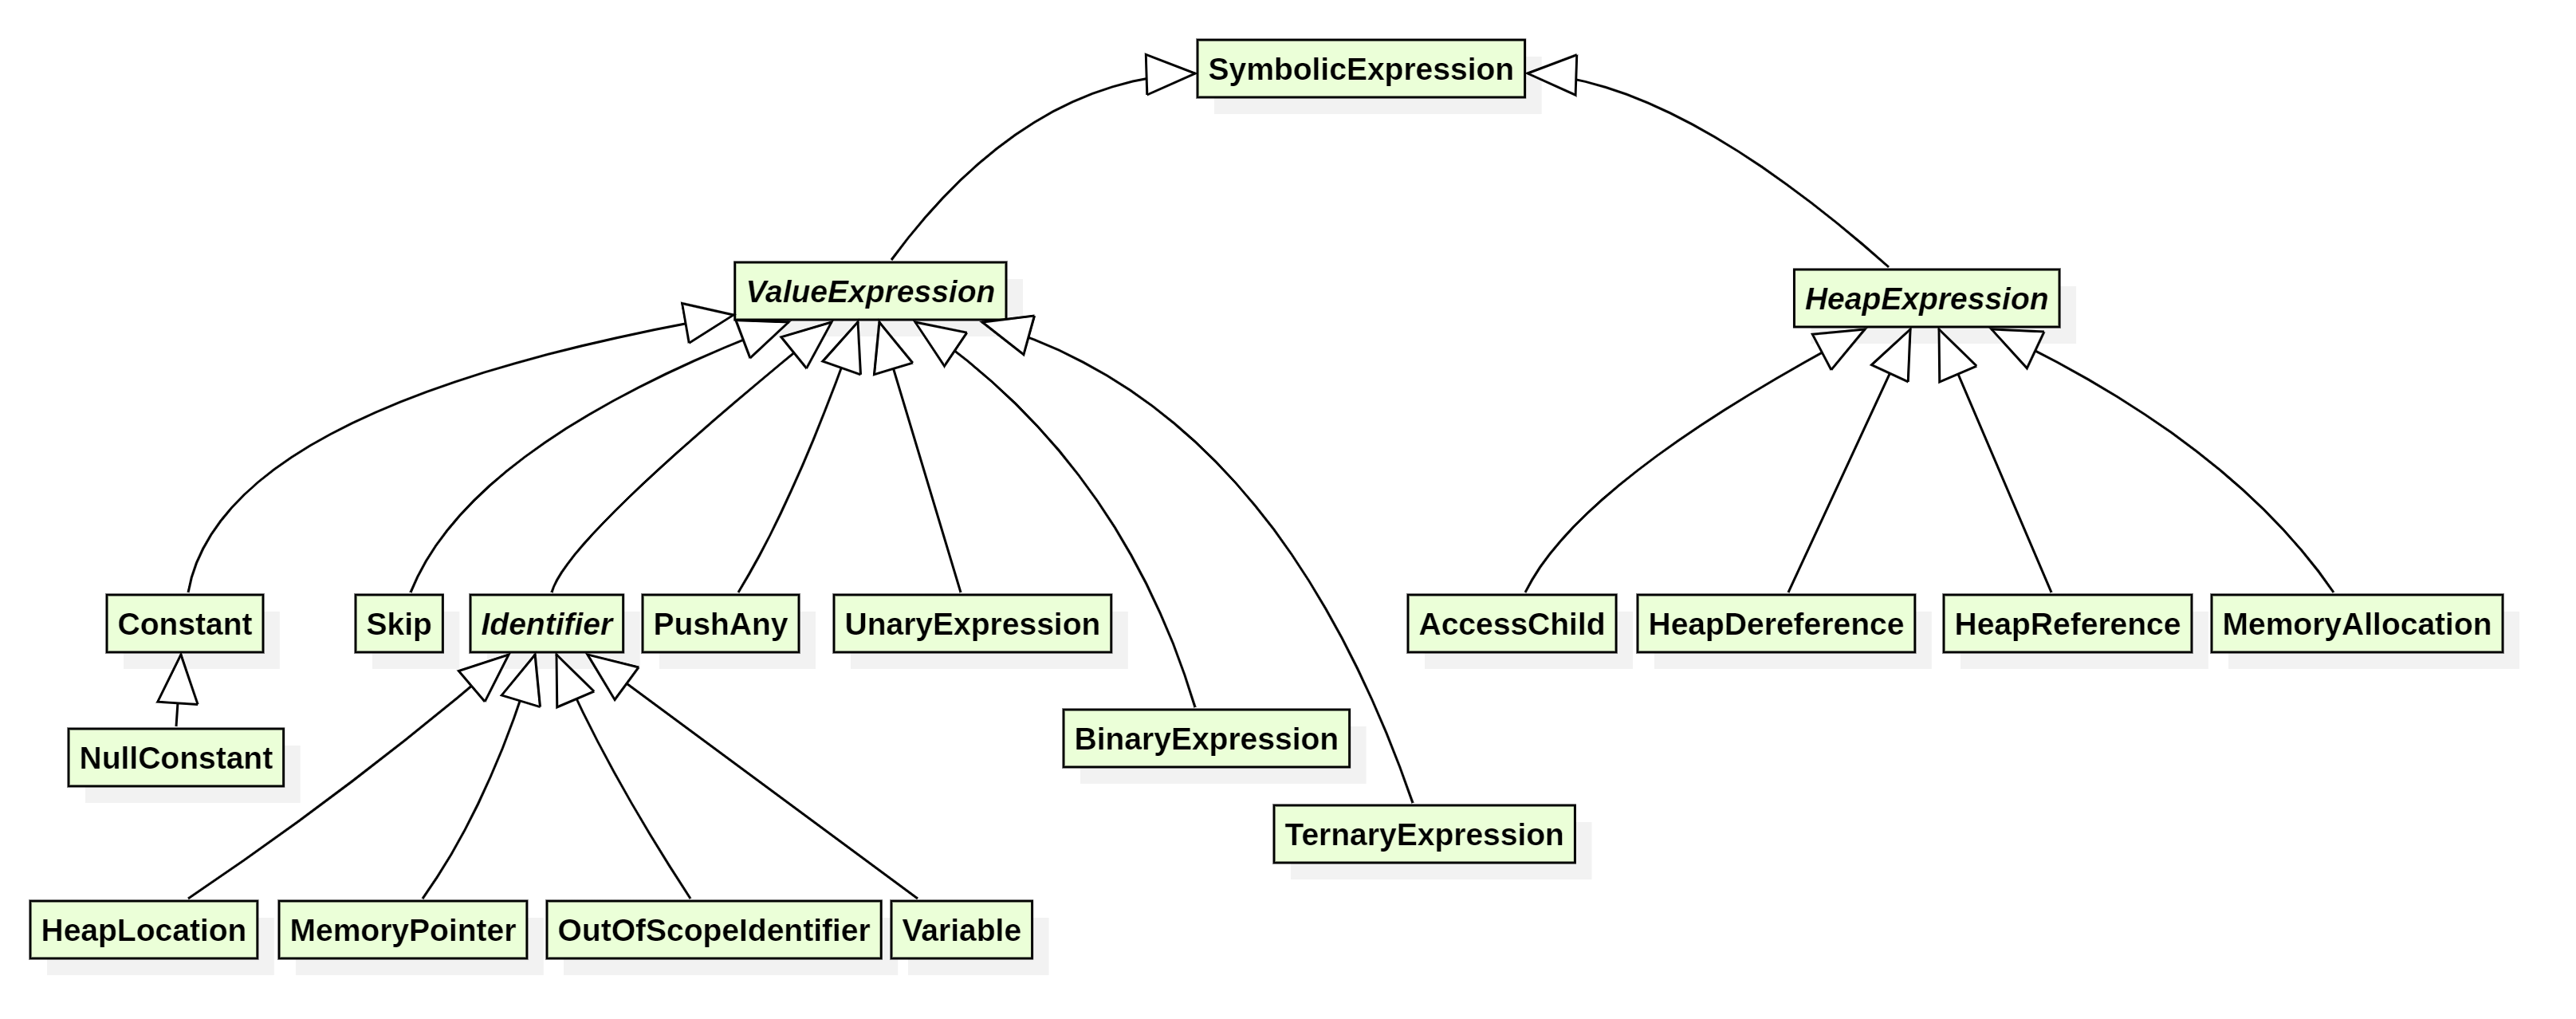
\includegraphics[width=0.9\textwidth]{Immagini/gerarchiaSymbolicExpression.png}
	\caption{Gerarchia della classe \texttt{statement}}
	\label{fig:gerarchiaSymbolic}
\end{figure}


Per fare un esempio prendiamo in considerazione lo statement \texttt{x = a + b} in un linguaggio non tipato (come Python), in cui non sappiamo i tipi dei valori di \texttt{a} e \texttt{b}. Questo statement in LiSA può essere tradotto in due espressioni simboliche, una per le parte sinistra, ovvero un riferimento alla variabile \texttt{x}, che può essere ulteriormente processata dal dominio astratto che modula l'heap, e una per la parte destra e modella la semantica dell'addizione \texttt{a + b}. Questa può anche controllare i tipi delle due variabili di \texttt{a} e \texttt{b} a run-time e in alcuni casi generare una \texttt{SymbolicExpression} che rappresenta l'addizione tra interi (se le due variabili possono avere valori numerici interi) e in altri casi una che rappresenta la concatenazione di stringhe (se entrambe possono contenere stringhe), o qualsiasi altro tipo di operazione modellata tramite il \texttt{+} che dipende dalle caratteristiche dei suoi operandi.
Questa traduzione run-time degli \texttt{Statement} in più \texttt{SymbolicExpression} rende i CFG di LiSA dinamici e plastici, quindi capaci di rappresentare un grande numero di costrutti semantici e la possibilità di modellare le funzioni della maggior parte dei linguaggi. Il compito del front-end in LiSA sarà quello di trasformare un programma scritto in un qualsiasi linguaggio di programmazione in un insieme di CFG comprendibili a LiSA, fatti di \texttt{Statement} (anche language-specific) e \texttt{edge}, e capaci di simulare \textit{completamente} la semantica del programma originale.

\subsection{Domini astratti in LiSA}
Ora parleremo invece di come sono definiti in LiSA i domini astratti. Ogni dominio in LiSA implementa due interfacce: \texttt{SemanticDomain}, che rende il dominio capace di valutare l'esecuzione di \texttt{SymbolicExpression} su istanze di esso, e \texttt{Lattice}, che fornisce al dominio le caratteristiche di un reticolo. Ora vediamo queste due interfacce più nel dettaglio.

\subsubsection{\texttt{SemanticDomain}}\label{subsec:semanticDomain}
L'interfaccia \texttt{SemanticDomain} è parametrica all'istanza concreta D, agli \texttt{Identifier} I e alle \texttt{SymbolicExpression} E. Rappresenta un dominio che è capace di ragionare sulla semantica delle \texttt{SymbolicExpression} di tipo E su \texttt{Identifier} di tipo I. Un dominio semantico D deve implementare i seguenti metodi:
\begin{itemize}
\setlength\itemsep{0.1em}
    \item \texttt{D assign(I id, E exp)}: restituisce un istanza del dominio in cui viene assegnato il valore di \texttt{exp} ad \texttt{id};
    \item \texttt{D assume(E exp)}: restituisce una istanza del dominio in cui si assume che \texttt{exp} sia vera;
    \item \texttt{D forgetIdentifier(I id)}: restituisce una istanza del dominio in cui viene scordata qualsiasi informazione riguardante l'identificatore \texttt{id};
    \item \texttt{D forgetIdentifiers(Collection<I> ids)}: restituisce una istanza del dominio in cui viene scordata qualsiasi informazione riguardante gli identificatori \texttt{ids};
    \item \texttt{Satisfiability satisfies(E exp)}: resituisce un valore (tra \texttt{SATISFIED}, \texttt{UNKNOWN}, \texttt{NOT\_SATISFIED} e \texttt{BOTTOM}) che indica se la espressione \texttt{exp} è soddisfatta nel dominio corrente;
    \item \texttt{D smallStepSemantics(E exp)}: resitutisce una istanza del dominio modificata dagli effetti della espressione \texttt{exp};
\end{itemize}

\subsubsection{\texttt{Lattice}}\label{subsec:lattice}
L'interfaccia \texttt{Lattice} è parametrica all'istanza concreta L. Un reticolo in LiSA deve implementare questi metodi:
\begin{itemize}
\setlength\itemsep{0.1em}
    \item \texttt{boolean lessOrEqual(L other)}: questo metodo definisce l'ordine parziale del reticolo e restituisce \texttt{true} se l'oggetto su cui viene chiamato è in relazione con \texttt{other};
    \item \texttt{L lub(L other)}: definisce l'operazione di least upper bound e restituisce il lub tra questo oggetto e \texttt{other};
    \item \texttt{L glb(L other)}: definisce l'operazione di greatest lower bound e restituisce il glb tra questo oggetto e \texttt{other};
    \item \texttt{L top(L other)}: restituisce l'elemento \(\top\) del reticolo;
    \item \texttt{L bottom(L other)}: restituisce l'elemento \(\perp\) del reticolo;
    \item \texttt{L widening(L other)}: definisce l'operazione di widening del reticolo e restituisce il widening tra questo oggetto e \texttt{other};
    \item \texttt{L narrowing(L other)}: definisce l'operazione di narrowing del reticolo e restituisce il narrowing tra questo oggetto e \texttt{other} (di defualt il narrowing esegue il glb);
    \item \texttt{boolean isTop()}: restiuisce \texttt{true} se l'istanza su cui viene chiamata è l'elemento \(\top\);
    \item \texttt{boolean isBottom()}: restiuisce \texttt{true} se l'istanza su cui viene chiamata è l'elemento \(\perp\);
\end{itemize}
In LiSA sono definite alcune implementazioni base di reticoli con comportamenti simili. Innanzitutto è definita l'interfaccia \texttt{BaseLattice} che estende \texttt{Lattice}, la quale definisce i casi base comuni a tutti i reticoli (ovvero le relazioni tra gli oggetti e gli elementi \(\top\) e \(\perp\)). A partire da questa sono poi implementate le classi astratte che definiscono il \texttt{SetLattice<E>} e \texttt{InverseSetLattice<E>} visti nell'esempio \ref{ex:setLattice} e il \texttt{FunctionalLattice<K,E>}, parametrico al tipo K del dominio della funzione e al tipo E del codominio nonchè dominio di un reticolo, visto nell'esempio \ref{ex:functionalLattice}. 


\subsubsection{Lo stato dell'analisi in LiSA: \texttt{AnalysisState}}

Vediamo ora come LiSA organizza lo stato dell'analisi. Lo stato dell'analisi è l'oggetto che viene mappato ad ogni nodo del CFG e indica l'astrazione della semantica  concreta che si vuole approssimare in quel punto di programma (solitamente in LiSA è una astrazione della collecting semantics, ovvero la semantica che ci dice tutti i possibili valori della memoria in un dato punto di programma o equivalentemente l'insieme di tutti gli stati attraversabili durante l'esecuzione del programma). Lo stato dell'analisi è costruito modularmente bottom-up come mostrato in figura \ref{fig:analysisState}.

\begin{figure}{0.35\textwidth}
\centering
\tikzset{every picture/.style={line width=0.75pt}} %set default line width to 0.75pt  
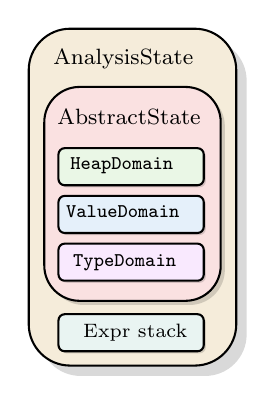
\begin{tikzpicture}[x=0.75pt,y=0.75pt,yscale=-1,xscale=1]
%uncomment if require: \path (0,300); %set diagram left start at 0, and has height of 300

%Rounded Rect [id:dp5259274252543102] 
\draw  [fill={rgb, 255:red, 245; green, 236; blue, 218 }  ,fill opacity=1 ][general shadow={fill={rgb, 255:red, 0; green, 0; blue, 0 }  ,shadow xshift=3.75pt,shadow yshift=-3.75pt, opacity=0.15 }] (20.67,194.89) .. controls (20.67,205.94) and (29.62,214.89) .. (40.67,214.89) -- (100.67,214.89) .. controls (111.71,214.89) and (120.67,205.94) .. (120.67,194.89) -- (120.67,72.59) .. controls (120.67,61.55) and (111.71,52.59) .. (100.67,52.59) -- (40.67,52.59) .. controls (29.62,52.59) and (20.67,61.55) .. (20.67,72.59) -- cycle ;
%Rounded Rect [id:dp40217338693406735] 
\draw  [fill={rgb, 255:red, 250; green, 225; blue, 225 }  ,fill opacity=1 ][general shadow={fill={rgb, 255:red, 0; green, 0; blue, 0 }  ,shadow xshift=1.5pt,shadow yshift=-1.5pt, opacity=0.15 }] (28.17,166.69) .. controls (28.17,176.08) and (35.78,183.69) .. (45.17,183.69) -- (96.17,183.69) .. controls (105.56,183.69) and (113.17,176.08) .. (113.17,166.69) -- (113.17,97.64) .. controls (113.17,88.25) and (105.56,80.64) .. (96.17,80.64) -- (45.17,80.64) .. controls (35.78,80.64) and (28.17,88.25) .. (28.17,97.64) -- cycle ;
%Shape: Rectangle [id:dp7147766556498871] 
\draw  [fill={rgb, 255:red, 249; green, 233; blue, 254 }  ,fill opacity=1 ][general shadow={fill={rgb, 255:red, 0; green, 0; blue, 0 }  ,shadow xshift=0.75pt,shadow yshift=-0.75pt, opacity=0.15 }] (35,159.14) .. controls (35,157.49) and (36.34,156.14) .. (38,156.14) -- (102,156.14) .. controls (103.66,156.14) and (105,157.49) .. (105,159.14) -- (105,171) .. controls (105,172.66) and (103.66,174) .. (102,174) -- (38,174) .. controls (36.34,174) and (35,172.66) .. (35,171) -- cycle ;
%Shape: Rectangle [id:dp6945641114766774] 
\draw  [color={rgb, 255:red, 0; green, 0; blue, 0 }  ,draw opacity=1 ][fill={rgb, 255:red, 229; green, 240; blue, 250 }  ,fill opacity=1 ][general shadow={fill={rgb, 255:red, 0; green, 0; blue, 0 }  ,shadow xshift=0.75pt,shadow yshift=-0.75pt, opacity=0.15 }] (35,136.14) .. controls (35,134.49) and (36.34,133.14) .. (38,133.14) -- (102,133.14) .. controls (103.66,133.14) and (105,134.49) .. (105,136.14) -- (105,148) .. controls (105,149.66) and (103.66,151) .. (102,151) -- (38,151) .. controls (36.34,151) and (35,149.66) .. (35,148) -- cycle ;
%Shape: Rectangle [id:dp6352913495307582] 
\draw  [fill={rgb, 255:red, 234; green, 247; blue, 230 }  ,fill opacity=1 ][general shadow={fill={rgb, 255:red, 0; green, 0; blue, 0 }  ,shadow xshift=0.75pt,shadow yshift=-0.75pt, opacity=0.15 }] (35,113.14) .. controls (35,111.49) and (36.34,110.14) .. (38,110.14) -- (102,110.14) .. controls (103.66,110.14) and (105,111.49) .. (105,113.14) -- (105,125) .. controls (105,126.66) and (103.66,128) .. (102,128) -- (38,128) .. controls (36.34,128) and (35,126.66) .. (35,125) -- cycle ;
%Shape: Rectangle [id:dp47123715282050216] 
\draw  [fill={rgb, 255:red, 233; green, 244; blue, 242 }  ,fill opacity=1 ][general shadow={fill={rgb, 255:red, 0; green, 0; blue, 0 }  ,shadow xshift=0.75pt,shadow yshift=-0.75pt, opacity=0.15 }] (35,193.14) .. controls (35,191.49) and (36.34,190.14) .. (38,190.14) -- (102,190.14) .. controls (103.66,190.14) and (105,191.49) .. (105,193.14) -- (105,205) .. controls (105,206.66) and (103.66,208) .. (102,208) -- (38,208) .. controls (36.34,208) and (35,206.66) .. (35,205) -- cycle ;


% Text Node
\draw (31,61) node [anchor=north west][inner sep=0.75pt]  [font=\footnotesize] [align=left] {AnalysisState};
% Text Node
\draw (33,90) node [anchor=north west][inner sep=0.75pt]  [font=\footnotesize] [align=left] {AbstractState};
% Text Node
\draw (39.2,113.2) node [anchor=north west][inner sep=0.75pt]   [align=left] {{\scriptsize \texttt{HeapDomain}}};
% Text Node
\draw (37.2,136.2) node [anchor=north west][inner sep=0.75pt]   [align=left] {{\scriptsize \texttt{ValueDomain}}};
% Text Node
\draw (40.6,159.8) node [anchor=north west][inner sep=0.75pt]   [align=left] {{\scriptsize \texttt{TypeDomain}}};
% Text Node
\draw (45.4,193.4) node [anchor=north west][inner sep=0.75pt]   [align=left] {{\scriptsize Expr stack}};
\end{tikzpicture}
    \caption{Architettura dello stato dell'analisi in LiSA}
    \label{fig:analysisState}
\end{figure}

La classe che definisce lo stato dell'analisi è \texttt{AnalysisState}. \'E formato da due componenti: un \texttt{AbstractState} e lo stack delle espressioni, ovvero l'insieme di \texttt{SymbolicExpression} che rimangono sullo stack dopo il calcolo di una espressione (è importante notare che questa è solo una visione sommaria dell'\texttt{AnalysisState}). Il principale compito di questa classe è quello però di fare da wrap tra l'\texttt{AbstractState} e informazioni semantiche aggiuntive utili al raggiungimento del fix-point durante il calcolo dell'analisi. L'\texttt{AnalysisState} implementa entrambe le interfacce mostrate prima (\hyperref[subsec:lattice]{\texttt{Lattice}} e \hyperref[subsec:semanticDomain]{\texttt{SemanticDomain}}) rendendolo un oggetto sia capace di ragionare sulla semantica delle espressioni simboliche che un sistema ordinato con le caratteristiche di un reticolo. Ogni sua componente, scendendo gerarchicamente nella struttura, implementa queste due interfacce. L'\texttt{AbstractState} è l'astrazione dello stato della memoria e, come si vede dall'immagine, è composto da tre sotto-domini (ognuno dei quali implementa le interfacce \hyperref[subsec:lattice]{\texttt{Lattice}} e \hyperref[subsec:semanticDomain]{\texttt{SemanticDomain}}): 
\begin{itemize}
\setlength\itemsep{0.1em}
    \item un \texttt{HeapDomain} che è responsabile di tracciare l'evoluzione dello stato della memoria dinamica durante l'esecuzione. Opera prima del \texttt{ValueDomain} e risolve gli indirizzi traducendo le espressioni simboliche e rinominando le variabili in modo tale che il \texttt{ValueDomain} possa comprenderle e si preocccupi \textit{solamente} di tracciarne le proprietà;
    
    \item un \texttt{ValueDomain} che è responsabile di tracciare proprietà astratte (come per esempio il valore astratto) delle variabili (possibilmente pre-processate e riscritte prima dall'\texttt{HeapDomain}) del programma. In LiSA è possibile definire \texttt{ValueDomain} sia relazionali (come i Polyhedra) sia non. Per quest'ultimi è definito dentro LiSA una classe base chiamata \texttt{Environment} che estende  \texttt{FunctionalLattice<Identifier, L>} ed implementa \texttt{SemanticDomain}, ed è capace di tracciare un valore del dominio astratto \texttt{L} (che può essere per esempio un Interval, un Sign, un Modulo) ad ogni identificatore tenuto in memoria. Va sottolineato che il dominio \texttt{L} di un \texttt{Environment} ha si la struttura reticolare, ed estende \texttt{Lattice}, e può anche ragionare semanticamente sulle \texttt{SymbolicExpression} senza però implementare \texttt{SemanticDomain}. Infatti per il caso specifico dei domini non-relazionali gestiti tramite \texttt{Environment} il dominio astratto si costruirà attraverso l'interfaccia \texttt{NonRelationalDomain} che ha solo un sottoinsieme dei metodi di \texttt{SemanticDomain}. Per capire perchè pensiamo ai metodi \texttt{assign}, \texttt{forgetIdentifier/s} in \texttt{SemanticDomain}. La definizione di questi metodi, potenzialmente, è uguale per tutti i dominio non-relazionali, ed infatti di queste se ne prende carico la classe \texttt{Environment}, lasciando alla creazione dei domini astratti non-relazionali solo la necessità di definire: (i) le operazioni riguardanti la struttura reticolare del dominio (lub, glb, lessOrEqual, \(\cdots\)), e (ii) la logica per la valutazione delle espressioni simboliche;
    
    \item un \texttt{TypeDomain} che è un \texttt{ValueDomain} che associa ad ogni variabile l'insieme dei possibili tipi a run-time delle variabili. Questa può essere usata durante l'analisi per generare espressioni simboliche specifiche a seconda dei tipi delle variabili coinvolte nello statement;
\end{itemize}

L'\texttt{AbstractState} principlamente fa quindi da coordinatore tra l'\texttt{HeapDomain} e il \texttt{ValueDoamin}, passando all'ultimo le espressioni tradotte e gli identificatori trasformati dal primo quando i due mondi devono comunicare e invece compartizzando e separando i due domini quando le espressioni riguardano solo su uno dei due.

\subsection{Calcolo del fix-point in LiSA}
Abbiamo visto nel capitolo [??] che fare interpretazione astratta (sezione [??]) non significa altro che trovare una soluzione ad un sistema di equazioni costruito a partire dal CFG del programma. Tutte le soluzioni del sistema sono per definizione suoi fix-point e quindi cercare la soluzione significa cercarne un fix-point (possibilmente il più preciso, ovvero il least fix-point). Come viene mostrato nell'articolo di Cousot [??] qualsiasi metodo caotico di risoluzione ci permette di ottenere una soluzione del sistema (non necessariamente la minima). Tra tutti questi metodi ci conviene usarne uno efficiente e che sfrutti la struttura del CFG in modo da velocizzare la convergenza verso un fix-point. L'algoritmo che viene utilizzato in LiSA per la risoluzione del sistema di equazioni è quello classico basato su working-set e prima delle mie modifiche seguiva la definizione in pseudo-codice fornita in \ref{alg:fixpointAsc}.

\begin{algorithm}[ht]
	\caption{Algoritmo per il calcolo del fix-point con working-set list con solo fase ascendente}
	\label{alg:fixpointAsc}
	\begin{algorithmic}
		\Statex
		%\Function{MST-Prim}{grafo G, funzione\_peso $\omega$, nodo\_radice r}\\
		\State{\textit{Q}: coda di priorita contenente tutti i vertici in \textit{V}}
		\For{ogni \textit{u} $\in$ V(G)}
		\Let{\textit{u.key}}{$\infty$}
		\Let{\textit{u.}$\pi$}{\textit{NIL}} 
		\EndFor
		\Let{\textit{r.key}}{0}
		\Let{\textit{Q}}{\textit{V(G)}}
		\While{\textit{Q} $\neq$ 0}
		\Let{\textit{u}}{EXTRACT-MIN(\textit{Q})}
		\For{ogni \textit{v} $\in$ \textit{G.Adj[u]}}
		\If{$v \in Q$ and $\omega(u,v) < v.key$}
		\Let{\textit{v.key}}{$\omega(u,v)$}
		\Let{\textit{v.}$\pi$}{\textit{v}}
		\EndIf
		\EndFor
		\EndWhile
		\State \Return{}
		%\EndFunction
	\end{algorithmic}
\end{algorithm}